\chapter{Steuerbereich \boldmath$U = [0,1]$}

Nach \autoref{ch:Aufgabe} besitzt die Steuerung $u(t)$ die Form:
\begin{align}
	u(t) = \exp\left(\frac{-\alpha}{\vartheta(t)}\right), &&\alpha > 0
\end{align}
Mit Umstellung nach der Temperatur folgt:
\begin{align}
	u(t) &= \exp\left(\frac{-\alpha}{\vartheta(t)}\right)			&&|\  \ln() \\
	\ln(u(t)) &= \frac{-\alpha}{\vartheta(t)}												&&|\  \cdot \vartheta(t) \\
	\ln(u(t)) \cdot \vartheta(t)&= -\alpha														&&|\  :  \ln(u(t)) \\
	\vartheta(t)&= \frac{-\alpha}{\ln(u(t))}
\end{align}
Durch die Forderung $\alpha > 0$, muss die Steuerung für sinnvolle Temperaturwerte immer aus dem Intervall $(0,1)$ kommen. Aus diesem Grund sind nachfolgend die Ergebnis aller numerischen Verfahren mit dem geänderten Steuerbereich $U = [0,1]$ aufgezeigt.
\begin{figure}[h!]
	\centering
	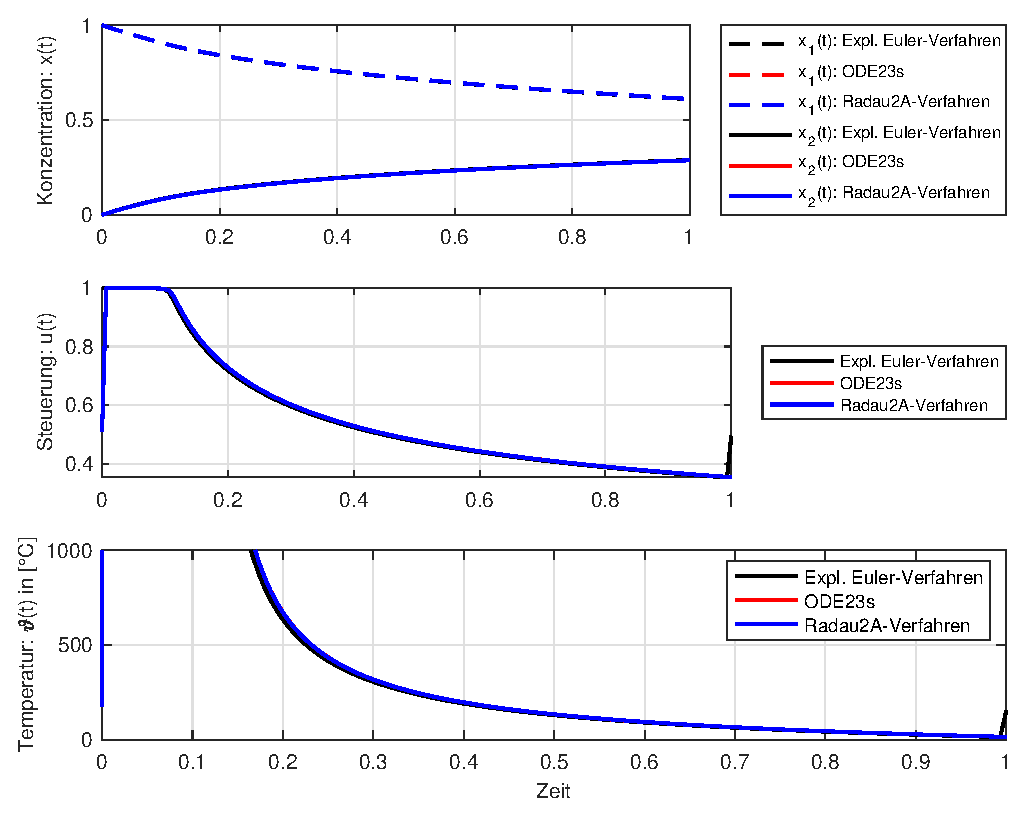
\includegraphics[width=1\textwidth]{images/CompareDirect_Method_U1}
	\caption{Direkte Verfahren mit $U=[0,1]$ und $\alpha = 300$: Vergleich}
	\label{fig:CompareDisk_U1}
\end{figure}

\begin{figure}[h!]
	\centering
	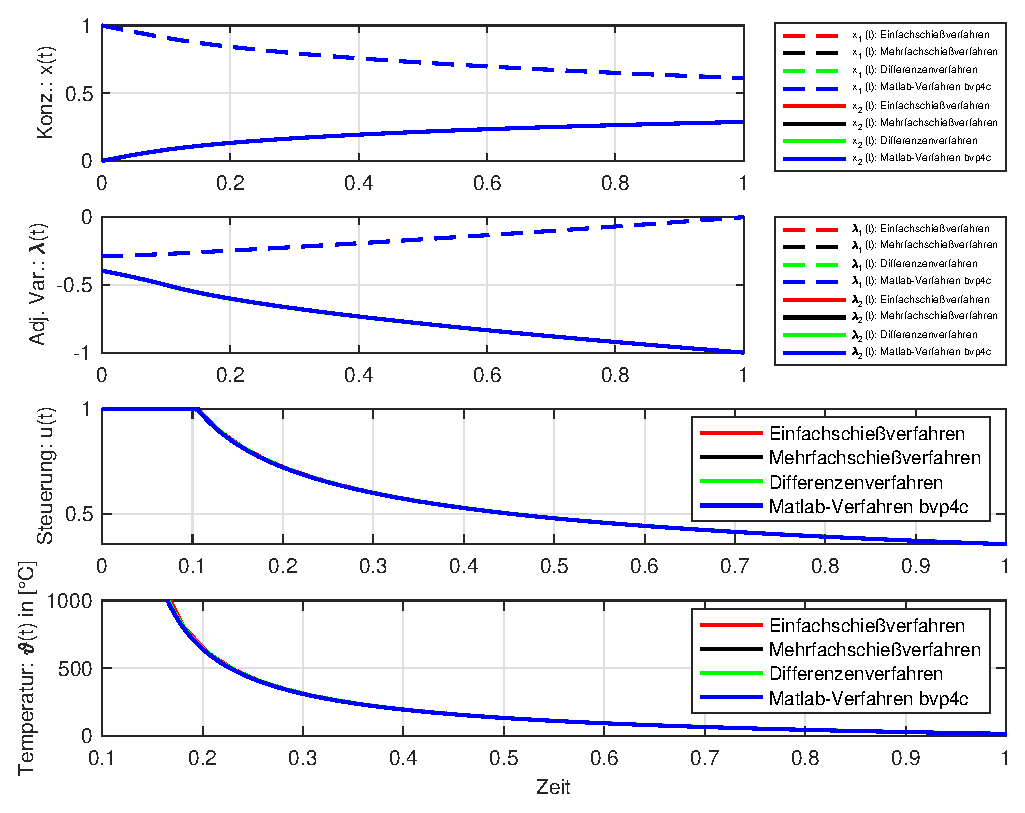
\includegraphics[width=1\textwidth]{images/CompareIndirect_Method_U1}
	\caption{Indirekte Verfahren mit $U=[0,1]$ und $\alpha = 300$: Vergleich}
	\label{fig:CompareBound_U1}
\end{figure}

\chapter{Zweifach stetige Differenzierbarkeit von \boldmath$H(u)$}\label{chap:A2}
\subsubsection*{Einfache stetige Differenzierbarkeit}
Der Nachweis der einfachen Differenzierbarkeit von $H(u)$ erfolgt anhand einer Existenzuntersuchung des Differentialquotienten: 
\begin{zz}$ \forall u_0 \in U \text{ } \exists \text{ } H_u(u_0) := \lim\limits_{u \rightarrow u_0} \frac{H(u)-H(u_0)}{u-u_0}$
\end{zz}
\begin{proof}
	Sei $u_0 \in U$ beliebig aber fest, so gilt:
	\begingroup
	\allowdisplaybreaks[3]	
	\begin{align}
		&H_u(u_0)= \lim\limits_{u \rightarrow u_0} \frac{H(u)-H(u_0)}{u-u_0} \\
		& = \lim\limits_{u \rightarrow u_0} \frac{(-\lambda_1 + \lambda_2) \cdot x_1 \cdot (u-u_0) + (\lambda_1 - 3 \lambda_2) \cdot x_2 \cdot (u^2-u_0^2)}{(u-u_0)} \\
		& = \lim\limits_{u \rightarrow u_0} \frac{(-\lambda_1 + \lambda_2) \cdot x_1 \cdot (u-u_0) + (\lambda_1 - 3 \lambda_2) \cdot x_2 \cdot (u-u_0) \cdot (u+u_0)}{(u-u_0)} \\
		& = \lim\limits_{u \rightarrow u_0} (-\lambda_1 + \lambda_2) \cdot x_1 + (\lambda_1 - 3 \lambda_2) \cdot x_2 \cdot (u+u_0)\\
		& = (-\lambda_1 + \lambda_2) \cdot x_1 + 2 \cdot (\lambda_1 - 3 \lambda_2) \cdot x_2 u_0
	\end{align}
	\endgroup
	%		& = \lim\limits_{u \rightarrow u_0} \frac{(-\lambda_1 + \lambda_2) \cdot x_1 \cdot (u-u_0) + (\lambda_1 - 3 \cdot \lambda_2) \cdot x_2 \cdot (u^2-u_0^2}{u-u_0)}	
	%
	%		& = \lim\limits_{u \rightarrow u_0} \frac{(-\lambda_1 + \lambda_2) \cdot x_1 \cdot u + (\lambda_1 - 3 \cdot \lambda_2) \cdot x_2 \cdot u^2 - (-\lambda_1 + \lambda_2) \cdot x_1 \cdot u_0 - (\lambda_1 - 3 \cdot \lambda_2) \cdot x_2 \cdot u_0^2}{u-u_0}
\end{proof}
Die Stetigkeit der ersten Ableitung lässt sich anhand des $\epsilon$-$\delta$ Kriteriums zeigen:
\begin{zz}
$ \forall\epsilon>0 \text{ } \exists \text{ } \delta>0: \forall u\in U: |u-u_0|<\delta \Rightarrow |H_u(u)-H_u(u_0)| < \epsilon $
\end{zz}
\begin{proof}
	Sei $\epsilon>0$, $\delta:=\frac{\epsilon}{|2\cdot(\lambda_1-3\lambda_2)\cdot x_2|}>0$, $|u-u_0|<\delta$, sowie $u \in U$. Dann gilt:
	\begin{align}
	|H_u(u) - H_u(u_0)| 
	& = |(2 \cdot (\lambda_1-3\lambda_2) \cdot x_2| \cdot |u-u_0|\\
	& < |(2 \cdot (\lambda_1-3\lambda_2) \cdot x_2| \cdot \delta 
	= \epsilon 
	\end{align}
%	\begin{align}
%	& |H_u(u) - H_u(u_0)| 
%	= |(2 \cdot (\lambda_1-3\lambda_2) \cdot x_2 \cdot (u-u_0)| \\
%	& = |(2 \cdot (\lambda_1-3\lambda_2) \cdot x_2| \cdot |u-u_0|\\
%	& < |(2 \cdot (\lambda_1-3\lambda_2) \cdot x_2| \cdot \delta \\
%	%& = |(2 \cdot (\lambda_1-3\lambda_2) \cdot x_2| \cdot \frac{\epsilon}{|(2 \cdot (\lambda_1-3\lambda_2) \cdot x_2|}  
%	= \epsilon 
%	\end{align}
\end{proof}
\subsubsection*{Zweifache stetige Differenzierbarkeit}
Analog zum vorherigen Abschnitt lässt sich die zweifache stetige Differenzierbarkeit zeigen. Zunächst wird wieder die Existenz des Differentialquotienten untersucht:
\begin{zz}
$\forall u_0 \in U \text{ } \exists \text{ } H_{uu}(u_0) := \lim\limits_{u \rightarrow u_0} \frac{H_u(u)-H_u(u_0)}{u-u_0}$
\end{zz}
\begin{proof}
Sei $u_0 \in U$ beliebig aber fest. Es gilt:
	\begin{align}
		H_{uu}(u_0) &= \lim\limits_{u \rightarrow u_0} \frac{H_u(u)-H_u(u_0)}{u-u_0} \\
		& = \lim\limits_{u \rightarrow u_0} \frac{2 \cdot (\lambda_1 - 3 \lambda_2) \cdot x_2 \cdot (u-u_0)}{(u-u_0)} \\
		& = \lim\limits_{u \rightarrow u_0} 2 \cdot (\lambda_1 - 3 \lambda_2) \cdot x_2 
		= 2 \cdot (\lambda_1 - 3 \lambda_2) \cdot x_2
	\end{align}
\end{proof}
Anschließend lässt sich mittels $\epsilon$-$\delta$-Kriterium die Stetigkeit der zweiten Ableitung zeigen: 
\begin{zz}
$ \forall\epsilon>0 \text{ } \exists \text{ } \delta>0: \forall u\in U: |u-u_0|<\delta \Rightarrow |H_{uu}(u)-H_{uu}(u_0)| < \epsilon $
\end{zz} 
\begin{proof}
	Sei $\epsilon>0$, $\delta>0$ beliebig aber fest, $|u-u_0|<\delta$ mit $u \in U$. Dann gilt:
	\begin{align}
	|H_{uu}(u)-H_{uu}(u_0)| 
	= |2\cdot(\lambda_1-3\lambda_2)\cdot x_2 -2\cdot(\lambda_1-3\lambda_2) \cdot x_2| 
	= 0 
	< \epsilon
	\end{align}
\end{proof}